\section{Formalizing EARS using Linear Temporal Logic}
\label{sec:formalization}

In this section we will use as running example the simplified requirements for
the operation of a controller of an engine system. The system includes a
\emph{main} engine, an \emph{auxiliary} engine and an \emph{oil pump} engine.
The sequence to start the machine is to first run the old pump engine; after 10 seconds start
the main engine; and after 5 more seconds start the auxiliary engine.
The \ears requirements for such a controller are depicted in
\fig\ref{fig:reqs_motor}.

\begin{figure}[!h]
\centering
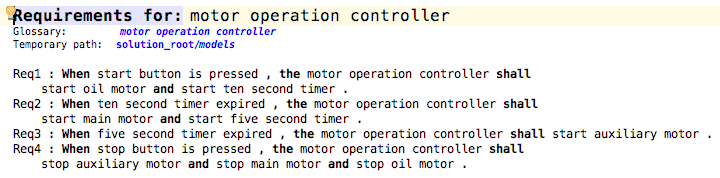
\includegraphics[width=.5\textwidth]{figures/motor_ears}
\caption{\ears requirements expressed in the \earsctrl environment}
\label{fig:reqs_motor}
\end{figure}

\begin{figure*}
\begin{tabular}{ |c|c|c| } 
 \hline
Ubiquitous & \textbf{The} $\langle$\emph{system}$\rangle$ \textbf{shall}
$\langle$\emph{response}$\rangle$ & $\mathbf{G}(response)$
\\
  \hline
Event-Driven & \textbf{When} $\langle$\emph{trigger}$\rangle$ \textbf{the}
$\langle$\emph{system}$\rangle$ \textbf{shall} $\langle$\emph{response}$\rangle$
& $\mathbf{G}(trigger\rightarrow \textbf{X}(response))$
\\
 \hline 
State-Driven &  \textbf{While} $\langle$\emph{in state}$\rangle$ \textbf{the}
$\langle$\emph{system}$\rangle$ \textbf{shall} $\langle$\emph{response}$\rangle$
& $\mathbf{G}(\text{\emph{in state}}\rightarrow response)$ \\
 \hline

Option &  \textbf{Where} $\langle$\emph{feature}$\rangle$ \textbf{the}
$\langle$\emph{system}$\rangle$ \textbf{shall} $\langle$\emph{response}$\rangle$
& $\mathbf{G}(\text{\emph{feature}}\rightarrow response)$ \\
 \hline
 
Complex &  \textbf{While} $\langle$\emph{in state}$\rangle$, \textbf{when}
$\langle$\emph{trigger}$\rangle$, \textbf{the} $\langle$\emph{system}$\rangle$
\textbf{shall} $\langle$\emph{response}$\rangle$ & $\mathbf{G}((\text{\emph{in
state}} \land \text{\emph{trigger}})\rightarrow \textbf{X}(response))$ \\
 \hline
 
Unwanted &  \textbf{If} $\langle$\emph{preconditions}$\rangle$
$\langle$\emph{trigger}$\rangle$, \textbf{the} $\langle$\emph{system}$\rangle$
\textbf{shall} $\langle$\emph{response}$\rangle$ &
$\mathbf{G}((\text{\emph{preconditions}} \land \text{\emph{trigger}})\rightarrow
\textbf{X}(response))$ \\
 \hline
 
\end{tabular}
\caption{Translation between \ears templates and \ltl}
\label{fig:translation_ears_ltl}
\end{figure*}

Let us now build a set of \ltl formulas that reflect the semantics of these
requirements. \ltl builds on propositional logic by adding temporal operators to
it. Formulas in \ltl are particularly appropriate to express properties of
runs of a reactive system, meaning how the state of that system should evolve
over time. For example, one may want to state that always, when a motor is on,
a thermostat is measuring its temperature. Or that, while the start button of a
car is pressed then the starter engine will assist in firing the main engine. Or
even, that eventually in the future the motor will stop. \ltl incorporates
operators to precisely describe these situations. Due to space limitations we
will refrain from formally introduce \ltl here, but will rather explain
the parts of it that are relevant to our presentation. Note that we do
assume basic familiarity with logical notations. \ltl was first introduced by
Pnueli in 1977~\cite{Pnueli77}.

By looking carefully at the example in \fig\ref{fig:reqs_motor} it is possible
to understand that all requirements are given in the form of \ears
\emph{event-driven} templates. Take for instance \textsf{Req1}. A
reasonable translation for it into \ltl would be as follows:

\begin{multline*}
\mathbf{G}(\text{\emph{start button pressed}} \rightarrow\\
\mathbf{X}(\text{\emph{start oil motor}}\land \text{\emph{start 10 sec timer}}))
\end{multline*}


The mathematical expression above reads as: \emph{globally},
during a run of the system (temporal operator $\mathbf{G}$), if the system
receives the \emph{start button} event, then in the \emph{next} moment
(temporal operator $\mathbf{X}$) the motor will be started as well a 10 second timer.

In the table in \fig\ref{fig:translation_ears_ltl} we present a generic set of
rules for transforming the \ears templates presented in~\cite{EARS09} into \ltl.
Note that all the transformation rules follow a similar pattern: for every state
in a run of the system some output is triggered, if a state satisfies a given
condition. In the \emph{ubiquitous} case, all states in the run have to produce
the response (enforced by the $\mathbf{G}$ operator). In the \emph{state-driven}
and \emph{option} case, the response is produced only if the state meets a
certain condition or a certain feature of the system is enabled.
The \emph{event-driven}, \emph{complex} and \emph{unwanted} patterns
are different in the sense that the response only appears in the moment
following the arrival of the trigger (as imposed by the $\mathbf{X}$ operator).
